\section{Designing Small-Scale Experiments}
\label{sec:designing-small-scale-experiments}

We synthesize our discussion into a methodology for small-scale experiments (\S\ref{sec:designing-small-scale-experiments:a-methodology-for-small-scale-experiments}). It emphasizes a holistic view because while regularities exist across scales, extrapolation hits statistical limits (\S\ref{sec:designing-small-scale-experiments:the-pitfalls-of-pure-extrapolation}). We demonstrate the approach on a case study from the literature: comparing pre-norm and post-norm transformers (\S\ref{sec:designing-small-scale-experiments:case-study-pre-norm-vs-post-norm-architectures}).

\subsection{A Methodology for Small-Scale Experiments}
\label{sec:designing-small-scale-experiments:a-methodology-for-small-scale-experiments}

Our approach relies on three facts:
%
\begin{enumerate}[noitemsep]
    \item with the pretraining data held fixed, capabilities depend on pretraining loss alone (\S\ref{sec:background:perplexity-capability-correspondence}),
    \item with rigorous hyperparameter tuning, scaling laws for pretraining extend to tiny scales (\S\ref{sec:estimating-small-scale-scaling-laws}),
    \item and as models scale, they grow far less sensitive to their hyperparameters (\S\ref{sec:understanding-the-hyperparameter-loss-surface-across-scales}).
\end{enumerate}
%
These principles prescribe a methodology for model-centric research: tune and measure at the small scale, understand how pretraining loss changes, then carry the winner up. The first fact says capability corresponds to perplexity, so we can evaluate models by their cost to obtain it; the second says pretraining laws can be observed at the small scale; and the third says the final scale-up is the easy part.

We expect these assumptions to hold, but should detect when they do not. The shape of small-scale experiments lets us do just that: we can exploit the anticipated structure, check when it fails, and turn those failures into useful diagnostics---for example, if either the noisy quadratic limit or scaling law fails to emerge then there is likely an issue with the hyperparameters, model, or implementation.

More than checking assumptions, however, these diagnostics build a qualitative understanding of how the loss surface scales. Such qualitative understanding is critical because quantitative approaches can compound small errors, even when based on sound structure. More than pure extrapolation, a holistic approach is necessary.

\subsection{The Pitfalls of Pure Extrapolation}
\label{sec:designing-small-scale-experiments:the-pitfalls-of-pure-extrapolation}


\begin{wrapfigure}{r}{0.48\textwidth}
    \centering
    \vspace{-1.3cm}
    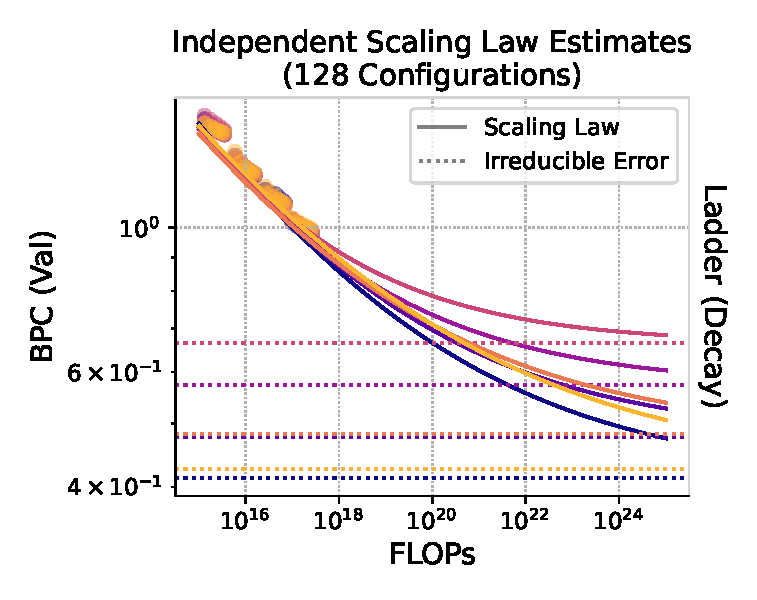
\includegraphics[width=0.43\textwidth]{figures/the-pitfalls-of-extrapolation.pdf}
    \caption{
        \emph{Despite good agreement near the data, extrapolation magnifies small differences due to sampling error.} We compare independent scaling law estimates, each based on 128 runs at 4M, 8M, 17M, and 34M parameters. Extrapolation eventually reflects the irreducible error, a quantity whose estimates vary greatly across different samples.
    }
    \label{fig:the-pitfalls-of-extrapolation}
    \vspace{-0.9 cm}
\end{wrapfigure}

Though scaling laws exist at small scales, their ability to extrapolate is another matter. We saw small-scale laws successfully extrapolate across an order of magnitude (\S\ref{sec:estimating-small-scale-scaling-laws}); however, what happens when we go further? \Cref{fig:the-pitfalls-of-extrapolation} 
% \sanae{update this if we add other panels to figure 1} 
illustrates how extrapolation magnifies the sampling error. Comparing independent estimates from different samples, we see the statistical noise: the irreducible error varies wildly across estimates.

If you compare models by extrapolating their scaling laws, at some point you are comparing their estimates of irreducible error. Such estimates are not reliable until the law begins to saturate. Scaling laws exist at small scales, and comparing them is useful; however, you cannot simply pick the model with the lowest final loss. The scaling law is there, but the statistical power is not. Instead, the law is much more reliable near the data.

\subsection{Case Study: Pre-Norm vs. Post-Norm Architectures}
\label{sec:designing-small-scale-experiments:case-study-pre-norm-vs-post-norm-architectures}

Where should normalization layers go in a transformer? The original placed them \emph{after} the residual connection (post-norm) \citep{Vaswani2017Attention}. This made training delicate, needing careful tuning. To stabilize training, \citet{baevski2018adaptiveinputrepresentationsneural} moved them \emph{before} the sublayer (pre-norm). A year later, an influential empirical study favored pre-norm in most settings yet, against today's practice, found post-norm better for high-resource machine translation \citep{nguyen-salazar-2019-transformers}. The matter only really settled when \citet{Xiong2020OnLayer} showed theoretically that pre-norm improves gradients at initialization. Pre-norm's advantage is most pronounced in deeper models, whose experiments are more expensive. Resolving it took nearly three years and a dedicated theoretical analysis. We will recover the answer from straightforward small-scale experiments.

A few well-separated scales should be far more informative than many nearby ones; we use three: two to fit the law, and one to validate it. For post-norm, we sample 511 configurations at 4M, 512 at 34M, and 128 at 134M; for pre-norm, we sample 128 at 4M, 34M, and 134M. We fit on the smaller two then evaluate on the largest one. This search is affordable because when parameters and data scale at the same rate compute is quadratic in model size. A single 1B-parameter run costs as much as 64 runs at 134M, 1{,}024 runs at 34M, or 65{,}536 runs at 4M. Thus, our experiment costs as much as a handful of billion parameter runs.

We now deepen our understanding of each architecture through a sequence of qualitative analyses. Each analysis is a diagnostic that asks a question and explores the structure we expect to find.

\paragraph{Diagnostic 1: have we tuned thoroughly?} If random search approaches the optimum, then the score distribution converges to a noisy quadratic as discussed in \Cref{sec:background:the-noisy-quadratic-limit} and established by \citet{lourie2025hyperparameter}. When the limit fails, it is likely the search missed the optimum.
% \footnote{
    % The noisy quadratic also enables deeper analyses such as confidence intervals for the best performance \citep{lourie2025hyperparameter}.
% } 
We visualize the limit for each architecture in \Cref{fig:noisy-quadratic-limit-for-prenorm-vs-postnorm}. For pre-norm it emerges readily; for post-norm it emerges too, but only deeper into the tail. This smaller asymptotic regime is an early indication of increased hyperparameter sensitivity. We seem to have located the optimum, but the tuning difficulty is itself our first finding: post-norm is sensitive to its hyperparameters, as the literature suggests.



\paragraph{Diagnostic 2: will scaling up be easy?} If larger models fail to become less sensitive to their hyperparameters, then transferring from small to large scales might fail as well. Therefore, we examine how sensitivity scales for the architectures at hand. \Cref{fig:sensitivity-across-scales-for-prenorm-vs-postnorm} compares the score distribution across scales for each. Both distributions move in the right direction, shifting mass towards the minimum as good configurations fill more of the space. For pre-norm the change is pronounced, growing a distinct peak at the optimum; for post-norm it is only slight, as a second peak lingers at a suboptimal value. Post-norm again exhibits tuning difficulty.



\paragraph{Diagnostic 3: does perplexity still track capabilities?} To evaluate by pretraining loss, it must correspond to capabilities (\S\ref{sec:background:perplexity-capability-correspondence}). This perplexity--capability correspondence should hold when pretraining data is fixed; still, the claim is easy to test as evaluating on a few tasks is much cheaper than pretraining the model. These tasks must show signal at small scales, like AI2 ARC (Easy) \citep{clark2018thinksolvedquestionanswering}. \Cref{fig:perplexity-capability-correspondence-for-prenorm-vs-postnorm} plots downstream accuracy vs. pretraining loss for several such tasks. Regardless of the architecture, all points fall on a common trend. Equal loss implies similar capabilities and a better pretraining law yields a more cost-effective model.

\paragraph{Diagnostic 4: do the scaling laws emerge?} To estimate the scaling laws, we adopt improvements from \S\ref{sec:estimating-small-scale-scaling-laws:the-impact-of-methodology}: tuning the hyperparameters per parameter--data budget and decaying the learning rate. Since extrapolation primarily reflects the noisy irreducible error (\S\ref{sec:designing-small-scale-experiments:the-pitfalls-of-pure-extrapolation}), we try fitting the laws jointly with tied irreducible error, as well as leaving them free to differ. \Cref{fig:validating-the-scaling-law} validates these scaling laws on the held-out scale. The free vs. joint laws extrapolate comparably. Pre-norm exhibits an excellent law, while post-norm's law is reasonable but could use improvement from further hyperparameter tuning. Again, hyperparameters present a challenge.



With a better understanding of each model, we now pool all sizes together and compare how the architectures scale. \Cref{fig:prenorm-vs-postnorm-compute-optimal-scaling} presents the result: pre-norm scales better over the range of sizes we explore. Remembering the statistical difficulty of extrapolating the scaling law (\S\ref{sec:designing-small-scale-experiments:the-pitfalls-of-pure-extrapolation}), we consider two kinds of comparisons. If we let each scaling have its own irreducible error, then the post-norm architecture appears to eventually outperform (beyond the scales we tested); however, if we share the irreducible error between the laws then the pre-norm architecture remains more efficient.

From a holistic viewpoint, post-norm was harder to tune at every turn. Even a better architecture in theory is worse in practice if we cannot find good hyperparameters. Beyond that, pre-norm scales better where the scaling laws are most reliable: near the data. Finally, when we assume both architectures reach the same final loss, pre-norm maintains its scaling advantage. These observations support pre-norm as the better choice.